Carrier Sense Multiple Access with Enhanced Collision Avoidance (CSMA/ECA)~\cite{CSMA_ECA} achieves less collisions and outperforms CSMA/CA in most typical scenarios. This is done by picking a deterministic backoff after each successful transmission. CSMA/E2CA introduces stickiness in the process by setting the number of times a deterministic backoff is used after each successful transmission, which accounts for a reduced convergence time towards a collision free state.

Stickiness can reduce the convergence time by orders of magnitude when the number of contenders $\eta$ is less or equal than the expectation of the random backoff used in CSMA/CA, $C$. The same constraint is valid for improvements in throughput, as can be appreciated in Figure~\ref{fig:throughput}.

\begin{figure}[htbp]
  \centering
  \includegraphics[width=0.7\linewidth, angle = -90]{figures/throughput/throughput.eps}
  \caption{Throughput and how it is affected when $\eta \geq C$
  \label{fig:throughput}}
\end{figure}

In Figure~\ref{fig:throughput}, when $\eta \geq C$ the system is overcrowded with contenders and the collision-free state is compromised. As more contenders are introduced, 